\subsection{Relational Streaming}\label{sec:sql} % Sherif

\begin{figure}[!h]
\begin{lstlisting}[morekeywords={Select,IStream,As,From,Range,Slide}]
Select IStream( Max(len) As mxl,
                MaxCount(len) As num,
                ArgMax(len, caller) As who )
From Calls[Range 24 Hours Slide 1 Minute]
\end{lstlisting}
\vspace*{-4mm}
\caption{\label{fig:cql}CQL code example.}
\end{figure}

\begin{figure}
\centerline{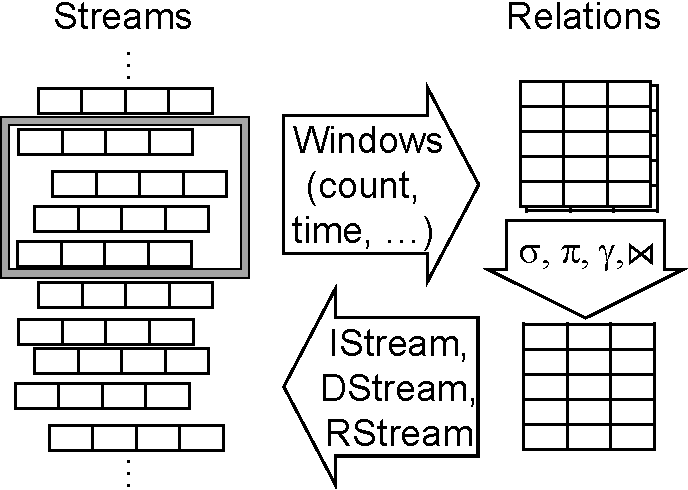
\includegraphics[scale=0.45]{cqlops.pdf}}
\vspace*{-4mm}
\caption{\label{fig:cqlops}CQL algebra operators.}
\end{figure}

In 2004, Arasu et al.\ at Stanford introduced \textsf{CQL} (for Continuous
Query Language)~\cite{arasu_widom_2004}. CQL has been designed as an
SQL-based declarative language for implementing continuous queries
against streams of data, such as the LinearRoad
benchmark~\cite{arasu_et_al_2004}. The design was influenced by the
\textsf{TelegraphCQ} system, which proposed an SQL-based language with a
focus on expressive windowing
constructs~\cite{chandrasekaran_et_al_2003}.
Dindar et al.~\cite{dindar2013modeling} presented a model to analyze  and understand the results of various window-based
queries (e.g., time- and tuple-based windows). Figure~\ref{fig:cql} illustrates a CQL code example that
uses a time-based sliding window (per minute within the last 24 hours) over
phone calls to return the maximum phone call length along with its
count and caller information.

The semantics of CQL are
based on two phases of data, \emph{streams} and \emph{relations}.
As Figure~\ref{fig:cqlops} illustrates, CQL
supports three classes of operators over these types. First,
\emph{stream-to-relation} operators freeze a stream into a relation.
These operators are based on
\emph{windows} that, at any point of time, contain a
historical snapshot of a recent portion of the stream. CQL includes
time-based and tuple-based windows, both with optional
partitioning. Second, \emph{relation-to-relation} operators, which
turn relations into another relation. These operators are expressed
using standard SQL syntax and come from traditional relational
algebra, such as select~($\sigma$), project~($\pi$),
group-by-aggregate~($\gamma$), and join~($\bowtie$).
Third, \emph{rela\-tion-to-stream} operators, which thaw a relation
back into a stream. CQL supports three operators of this class:
\texttt{IStream}, \texttt{DStream}, and \texttt{RStream} (to capture inserts, deletes, or the entire
relation).

Besides TelegraphCQ, another predecessor of CQL was
\textsf{GSQL}~\cite{cranor_et_al_2003}.  In addition to the standard SQL
operators (e.g., $\sigma$, $\pi$, $\gamma$,~$\bowtie$), GSQL supports
a \emph{merge} operator that combines streams from multiple sources in
order as specified by ordered attributes.  GSQL supports joins as long
as it can determine a window from ordered attributes and join predicates.

CQL has influenced the design of many systems, for example, \textsf{Microsoft
StreamInsight}~\cite{ali_et_al_2009} and \textsf{StreamSQL}~\cite{StreamSQL}.  Jain et al.\ described an
approach to unify two different proposed SQL extensions for
streams~\cite{jain_et_al_2008}. The first proposal, presented by
Oracle and based on CQL, used a time-based execution model that
provided a way to model simultaneity. The second proposal, presented
by \textsf{StreamBase}, used a tuple-based execution model that provided a way
to react to primitive events as soon as they are seen by the system.
Jain et al.\ captured ordering and simultaneity through partial orders
on batches of tuples using a new \emph{Spread} operator.  Zou et
al.\ showed how to turn a stream of queries into a stream query by
streaming their parameters~\cite{zou_et_al_2010}.  And Soul\'{e} et
al.~\cite{soule_et_al_2016} presented a formal type system and
small-step operational semantics for CQL via translation to a calculus
for stream processing named \texttt{Brooklet}~\cite{soule_et_al_2010}.

The design of CQL has been influenced by the temporal relational model introduced by Jensen and Sondgrass in  the early 90s~\cite{jensen1994temporal}. In this model, each temporal relation has two main dimensions: a valid time record and transaction time. Chandramouli et al.~\cite{chandramouli2012temporal} has built on top of this model by presenting \textsf{TiMR}, a framework that implements a time-oriented data processing approach using the MapReduce framework based on temporal queries.
